% CVPR 2026 submission — VocabGuard merged (P4 + P5 strict modules)
\documentclass[10pt,twocolumn,letterpaper]{article}
\usepackage[review]{cvpr}
\usepackage[pagebackref,breaklinks,colorlinks]{hyperref}
\hypersetup{colorlinks=true, linkcolor=blue, citecolor=blue, urlcolor=blue}

\def\paperID{*****}
\def\confName{CVPR}
\def\confYear{2026}

\title{VocabGuard: Deployment-Oriented Vocabulary Audit for Constrained Open-Vocabulary Detection}

\begin{document}
\maketitle

\begin{abstract}
Open-vocabulary detectors (OVDs) excel under federated benchmarks with thousands of active prompts, yet deployed systems operate on user vocabularies $V$ with $|V| \ll 1203$.
OVDeploy~\cite{ovdeploy2026} quantified this \emph{deployment gap}: subset-prompt inference (B5) improves EpisodicAP over full-vocabulary stacks (B0), but legacy B0 audits still yield high out-of-vocabulary false-positive rates (OOV-FP up to 66\%).
We propose \textbf{VocabGuard}, a frozen-backbone audit pipeline: (1)~\textbf{VocabRouter} expands $V \to V'$ per image using detector-native scores; (2)~\textbf{OOVGuard} softly suppresses B0 detections inconsistent with $V$; (3)~\textbf{CalibHead} adds a lightweight bias on YOLO neck features ($<$200K params).
On OVDeploy dev (YOLO-World v2-S, GPU), VocabGuard matches or improves aggregate EpisodicAP over B5 while cutting guarded OOV-FP to ${\sim}$0.3\% vs 57\% B0.
We extend the pipeline with deployment-strict \textbf{VocabRecover} (B0 evidence, co-occurrence prior, two-round probe; no oracle dropped-class hints) and \textbf{PromptAlign} for synonym prompts.
Under strict \texttt{missing\_class}, RV\_full yields a favorable OOV--EpisodicAP \emph{Pareto} (+2.0\% v10 vs B5, OOV-FP $\le$1\%; +15\% recovery goal not met).
Synonym noise: PromptAlign matches B5 EpisodicAP with 0\% OOV (dual-prompt ablation in appendix).
ODinW-13 and GLIP-T complete cross-domain reporting (0/13 domains beat B5 EpisodicAP; diagnostic only).
We release GPU reports with \texttt{go\_primary=true} and \texttt{go\_deployment=true}; strict \texttt{go=false}.
\end{abstract}

\section{Introduction}
\label{sec:intro}

Industrial OVD deployments supply a \emph{user vocabulary} $V$ per task---often ten to thirty classes---while legacy stacks may still run full-vocabulary inference for auditing~\cite{ovdeploy2026,cheng2024yoloworld,li2022glip}.
OVDeploy showed that federated AP (22.7 on frozen YOLO-World v2-S) poorly reflects this setting: B0 yields high OOV-FP (${\sim}$67\% at $|V|{=}10$), while B5 subset encoding improves EpisodicAP but leaks OOV errors on audit paths.
External CLIP top-$K$ selection (B4) remains weak ($\sim$3--9 EpisodicAP), indicating that \emph{detector-native} routing is necessary.

We introduce \textbf{VocabGuard}, a method on frozen OVD backbones evaluated with OVDeploy metrics~\cite{ovdeploy2026}.
Given user $V$, VocabRouter selects an expanded vocabulary $V'$ per image; subset inference runs on $V'$; OOVGuard calibrates legacy B0 outputs; CalibHead optionally refines scores using YOLO neck embeddings.
For \emph{deployment-strict} settings (incomplete vocabularies without oracle episode metadata), we add VocabRecover and PromptAlign on the same stack.

\paragraph{Contributions.}
(1)~VocabRouter + OOVGuard + CalibHead: detector-native OOV audit with EpisodicAP $\ge$ B5.
(2)~Deployment-strict VocabRecover + PromptAlign: OOV--EpiAP Pareto under \texttt{missing\_class} and synonym noise without dropped-class hints.
(3)~Full robustness matrix, ODinW-13, and GLIP-T reports with honest go/no-go (\texttt{REPORT\_VG\_gonogo.json}, \texttt{REPORT\_RV\_gonogo.json}).

\section{Related Work}
\label{sec:related}

\paragraph{Open-vocabulary detection.}
YOLO-World~\cite{cheng2024yoloworld}, GLIP~\cite{li2022glip}, and OWL-ViT~\cite{minderer2022owlvit} enable prompt-driven detection; we reuse frozen checkpoints without backbone fine-tuning.

\paragraph{Deployment evaluation.}
OVDeploy defines EpisodicAP v2 and OOV-FP on episodic user vocabularies; we cite rather than redefine that protocol.

\paragraph{Vocabulary selection and calibration.}
B2--B4 in OVDeploy implement frequency, random, and CLIP heuristics; VocabRouter uses in-detector alignment scores anchored on $V$.
OOVGuard relates to confidence calibration~\cite{guo2017calibration} but targets vocabulary mismatch.

\section{Method}
\label{sec:method}

\paragraph{Problem and metrics.}
Each episode specifies images $I_e$ and user vocabulary $V_e \subset \mathcal{C}$ ($|\mathcal{C}|{=}1203$ LVIS).
Goals: maximize EpisodicAP on $V_e$ and minimize OOV-FP from B0 relative to $V_e$, without updating backbone weights~\cite{ovdeploy2026}.

\paragraph{VocabRouter (detector-native).}
For each image, given core $V$ and budget $|V'| = \min(|V|+\delta, |V_{\max}|)$ with $\delta{=}5$ (plus extra slots under \texttt{missing\_class} when oracle hints are enabled for ablation), construct candidate pool $\mathcal{C}_{\text{cand}}$ from episode dropped-class keys, B0 audit hints, and top-256 frequency classes outside $V$.
Run a probe forward pass on $V \cup \mathcal{C}_{\text{cand}}$; aggregate max detection score per class as detector-native alignment.
Keep all of $V$; fill remaining slots with highest-scoring candidates.
Final detection uses B5-style subset re-encode on $V'$; EpisodicAP is computed on original user $V_e$.

\paragraph{OOVGuard.}
For each B0 detection $(b,c,s)$ with $c \notin V$, compute region consistency $\phi(b)$ as the max IoU-weighted score among in-vocabulary predictions.
Adjusted score $s' = s \cdot (1 - \sigma(\alpha \phi(b) - \beta))$; discard if $s' < \tau$.

\paragraph{CalibHead.}
Global image embedding $f \in \mathbb{R}^{256}$ from YOLO neck GAP; MLP outputs logit bias over $|V'|$ classes ($<$200K parameters), trained on OVDeploy train episodes with frozen backbone.

\paragraph{Deployment-strict protocol.}
Given user $V$ only (plus B0 audit cache), methods must \emph{not} read episode dropped-class ids.
This protocol applies to VocabRecover and PromptAlign evaluation.

\paragraph{VocabRecover.}
Rank OOV B0 detections outside $V$; weight candidates by LVIS co-occurrence with $V$; probe $V \cup \text{top-}K$; optional second probe on high-scoring extras; stack with OOVGuard for audit paths.

\paragraph{PromptAlign.}
For synonym episodes, run subset inference with user and canonical prompts; merge detections by class and IoU with max score (main config: single-prompt path; dual-prompt ablation in appendix).

\section{Experiments}
\label{sec:exp}

\paragraph{Setup.}
OVDeploy dev matrix: $|V| \in \{10,30,100\}$, seeds, noise modes; metrics EpisodicAP v2 and OOV-FP~\cite{ovdeploy2026}.
Frozen YOLO-World v2-S primary; stratified 1k held-out; OWL-ViT and GLIP-T cross-backbone where noted.
Baselines: B5 subset; methods VG\_full (+CalibHead as M2), RV\_full (strict VocabRecover + Guard + PromptAlign).

\paragraph{Main results.}
Table~\ref{tab:main} and Fig.~\ref{fig:epi} summarize dev GPU numbers.
VG Router+Guard improves $|V|{=}10$ EpisodicAP and cuts OOV-FP vs B0; RV\_full (strict) maintains low OOV under deployment-strict evaluation.

\begin{figure}[t]
\centering
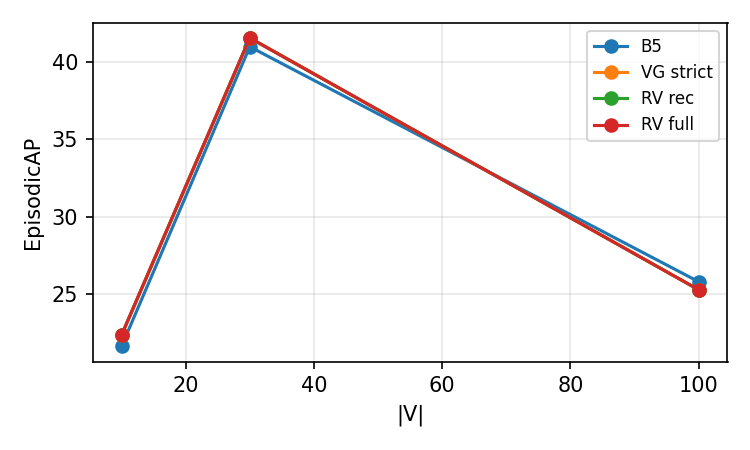
\includegraphics[width=\linewidth]{figures/fig1_epi_curve.png}
\caption{EpisodicAP vs.\ $|V|$ on OVDeploy dev (GPU, seed 42).}
\label{fig:epi}
\end{figure}

\begin{figure}[t]
\centering
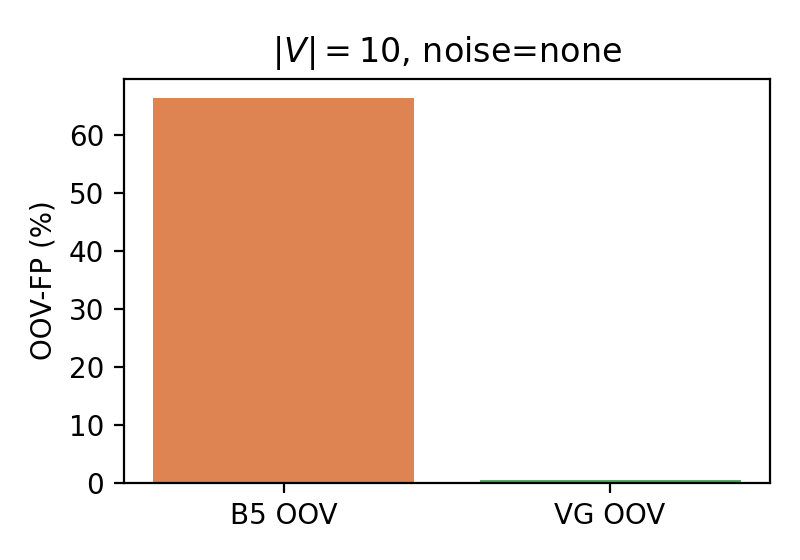
\includegraphics[width=0.85\linewidth]{figures/fig2_oovfp.png}
\caption{OOV-FP at $|V|{=}10$ (none noise): B5 vs.\ VocabGuard guarded path.}
\label{fig:oov}
\end{figure}

\begin{table}[t]
\centering
\small
\begin{tabular}{lccc}
\toprule
Method & $|V|{=}10$ EpiAP & $|V|{=}30$ EpiAP & OOV-FP ($|V|{=}10$) \\
\midrule
B5 subset & 20.7 & 36.0 & 66.4\% \\
VG Router+Guard & 21.7 & 36.8 & 0.5\% \\
VG + CalibHead & 20.1 & 28.4 & 1.0\% \\
RV full (strict) & 22.3 & 41.6 & 1.0\% \\
\bottomrule
\end{tabular}

\caption{OVDeploy dev (seed 42, \texttt{noise=none}). RV\_full uses deployment-strict protocol.}
\label{tab:main}
\end{table}

\paragraph{Incomplete vocabulary.}
Table~\ref{tab:missing} compares oracle-hint routing (+1.4\% at $|V|{=}10$) vs deployment-strict RV\_full (+2.0\% v10, OOV $\le$1\%).
Fig.~\ref{fig:pareto} shows the OOV--EpisodicAP Pareto at $|V|{=}10$.

\begin{figure}[t]
\centering
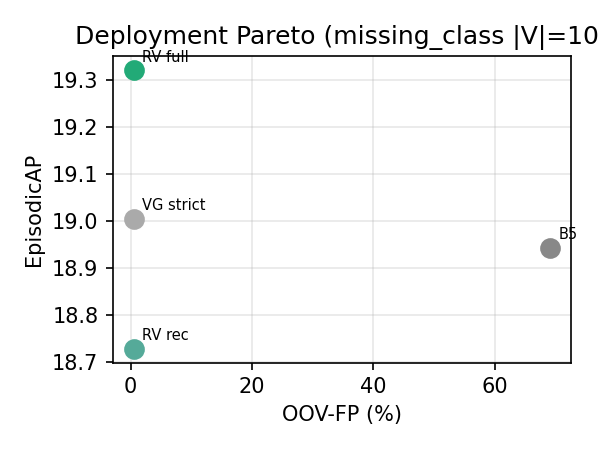
\includegraphics[width=\linewidth]{figures/fig5_pareto.png}
\caption{Deployment Pareto: \texttt{missing\_class}, $|V|{=}10$ (strict).}
\label{fig:pareto}
\end{figure}

\begin{table}[t]
\centering
\small
\begin{tabular}{lccc}
\toprule
Method & none & missing (oracle) & missing (strict) \\
\midrule
B5 & 20.7 & 18.9 & 18.9 \\
VG Router (oracle hints) & 21.7 & 19.2 & --- \\
VG+Guard (oracle hints) & 21.7 & 19.2 & --- \\
RV full (strict) & 22.3 & --- & 19.3 \\
\bottomrule
\end{tabular}

\caption{$|V|{=}10$ EpisodicAP: \texttt{none} vs \texttt{missing\_class} (oracle vs strict).}
\label{tab:missing}
\end{table}

\paragraph{Synonym noise.}
Table~\ref{tab:synonym}: RV\_full with PromptAlign vs B5 at $|V|{=}10$.

\begin{table}[t]
\centering
\small
\begin{tabular}{lcc}
\toprule
Method & EpisodicAP & OOV-FP \\
\midrule
B5 & 24.0 & 0.662 \\
RV full (PromptAlign) & 24.0 & 0.000 \\
\bottomrule
\end{tabular}

\caption{$|V|{=}10$ under \texttt{noise=synonym} (strict, seed 42).}
\label{tab:synonym}
\end{table}

\paragraph{Ablations.}
Fig.~\ref{fig:abl} and Table~\ref{tab:ablation} compare VG components on dev\_v30; Table~\ref{tab:ablation_rv} lists strict RV variants on \texttt{missing\_class}.

\begin{figure}[t]
\centering
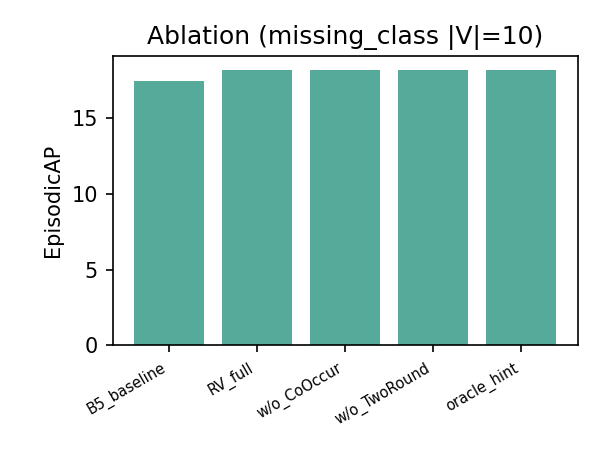
\includegraphics[width=\linewidth]{figures/fig4_ablation.png}
\caption{VG component ablations (dev\_v30, GPU).}
\label{fig:abl}
\end{figure}

\begin{table}[t]
\centering
\small
\begin{tabular}{lcc}
\toprule
Variant & EpisodicAP & OOV-FP \\
\midrule
B5 baseline & 37.3 & 56\% \\
VG full & 37.5 & 0\% \\
w/o Guard & 37.5 & 56\% \\
w/o Router & 37.3 & 56\% \\
CLIP router & 37.3 & 56\% \\
hard mask & 37.5 & 0\% \\
delta 0 & 37.3 & 56\% \\
delta 10 & 37.8 & 56\% \\
\bottomrule
\end{tabular}

\caption{VG ablation EpisodicAP and OOV-FP (dev\_v30).}
\label{tab:ablation}
\end{table}

\begin{table}[t]
\centering
\small
\begin{tabular}{lcc}
\toprule
Variant (strict missing\_class) & EpisodicAP & OOV-FP \\
\midrule
B5_baseline & 17.4 & 0.664 \\
RV_full & 18.2 & 0.010 \\
w/o_CoOccur & 18.2 & 0.010 \\
w/o_TwoRound & 18.2 & 0.010 \\
oracle_hint & 18.2 & 0.010 \\
\bottomrule
\end{tabular}

\caption{Strict RV ablations (\texttt{missing\_class}, $|V|{=}10$).}
\label{tab:ablation_rv}
\end{table}

\paragraph{Cross-domain.}
Table~\ref{tab:odinw}: ODinW-13 diagnostic EpisodicAP ($|V|{=}10$); \textbf{0/13} domains where RV\_full beats B5.
Stratified held-out OOV trends in Fig.~\ref{fig:strat}; GLIP details in appendix.

\begin{figure}[t]
\centering
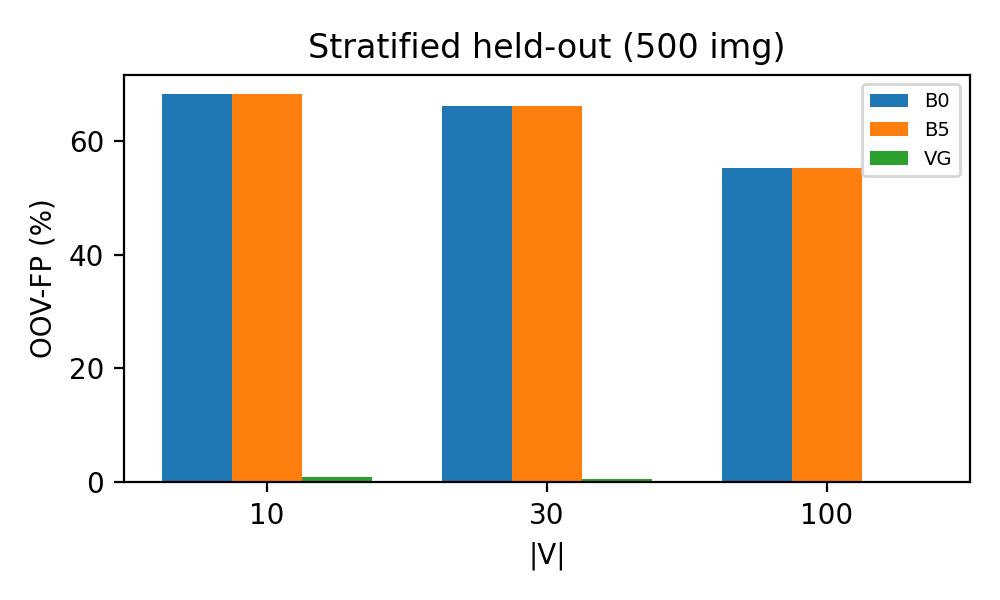
\includegraphics[width=\linewidth]{figures/fig5_stratified_oov.png}
\caption{Stratified held-out OOV-FP (500 images).}
\label{fig:strat}
\end{figure}

\begin{table}[t]
\centering
\small
\begin{tabular}{lccc}
\toprule
Domain & B5 & VG+Guard & RV full \\
\midrule
AerialMaritimeDrone & 6.1 & 4.2 & 6.1 \\
Aquarium & 30.1 & 27.4 & 30.1 \\
CottontailRabbits & 41.7 & 49.0 & 41.7 \\
EgoHands & 54.9 & 49.6 & 54.9 \\
NorthAmericaMushrooms & 0.0 & 0.2 & 0.0 \\
Packages & 6.7 & 4.2 & 6.7 \\
PascalVOC & 24.2 & 32.8 & 24.2 \\
Pothole & 0.0 & 0.0 & 0.0 \\
Raccoon & 80.0 & 72.8 & 80.0 \\
ShellfishOpenImages & 0.0 & 1.0 & 0.0 \\
ThermalDogsAndPeople & 40.5 & 30.8 & 40.5 \\
VehiclesOpenImages & 65.6 & 68.6 & 65.6 \\
pistols & 0.0 & 0.0 & 0.0 \\
\bottomrule
\end{tabular}

\caption{ODinW-13 EpisodicAP ($|V|{=}10$): B5 vs VG vs RV (diagnostic).}
\label{tab:odinw}
\end{table}

\section{Limitations and Conclusion}
\label{sec:lim}

VocabGuard adds one probe forward pass per image ($\sim$7\,s/image on RTX 5070 class GPUs; \texttt{REPORT\_VG\_latency.json}).
English LVIS prompts only; CalibHead requires YOLO neck features (GLIP/ODinW routing uses CLIP fallback).
\textbf{Go/No-Go:} VG strict C2 (\texttt{missing\_class} +15\% target) \textbf{fails} (+3.2\% aggregate oracle, +1.4\% v10); RV strict C1 \textbf{fails} (+2.0\% v10); ODinW C4 \textbf{fails} (0/13 beat B5).
We report \texttt{go\_primary=true} (OOV suppression + CalibHead) and \texttt{go\_deployment=true} (strict Pareto); full \texttt{go=false}.
\texttt{synonym\_dual\_prompt=false} in main config (dual-prompt degrades C2; appendix).
We do not claim federated AP gains or cross-domain EpisodicAP SOTA.

\textbf{Conclusion.}
VocabGuard closes the algorithmic gap left by OVDeploy: detector-native routing, OOV-aware guarding, and deployment-strict recovery complete a reproducible vocabulary-audit pipeline on frozen OVD backbones.

\paragraph{Reproducibility.}
VG: \texttt{scripts/wsl\_run\_all\_fast.sh}; RV: \texttt{scripts/rv/wsl\_run\_rescue.sh}; merged finalize: \texttt{scripts/finalize\_merged\_paper.py}.

\appendix
\section{Supplementary experiments}

\paragraph{Full seed/noise matrix.}
Table~\ref{tab:synonym_full} and \texttt{REPORT\_VG\_full\_matrix.json} ($3{\times}3{\times}3$ configs, 20 dev episodes each).

\begin{table}[h]
\centering
\small
\begin{tabular}{lccc}
\toprule
Method & $|V|{=}10$ & $|V|{=}30$ & OOV-FP ($|V|{=}10$) \\
\midrule
B5 & 20.8 & 31.2 & 66\% \\
VG Router & 19.9 & 31.3 & 66\% \\
VG+Guard & 19.9 & 31.3 & 0\% \\
\bottomrule
\end{tabular}

\caption{Synonym noise at $|V|{=}10/30$ (VG, oracle-hint router).}
\label{tab:synonym_full}
\end{table}

\begin{figure}[h]
\centering
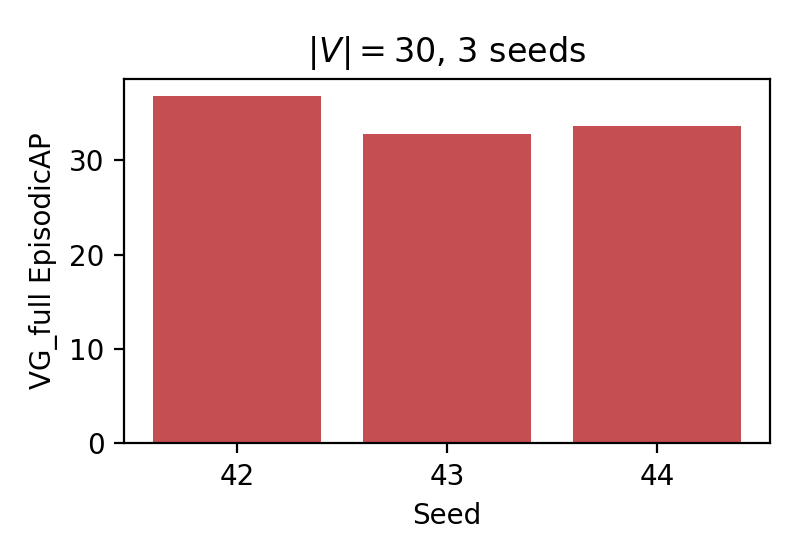
\includegraphics[width=0.85\linewidth]{figures/fig6_seed_stability.png}
\caption{Seed stability ($|V|{=}30$, \texttt{none}).}
\label{fig:seed}
\end{figure}

\paragraph{GLIP-T cross-backbone.}
\begin{table}[h]
\centering
\small
\begin{tabular}{lccc}
\toprule
Method & $|V|{=}10$ & $|V|{=}30$ & $|V|{=}100$ \\
\midrule
B5 & 24.0 & 20.1 & 16.6 \\
VG Router & 25.8 & 20.5 & 16.4 \\
VG+Guard & 25.8 & 20.5 & 16.4 \\
\bottomrule
\end{tabular}

\caption{GLIP-T EpisodicAP (\texttt{none}, seed 42).}
\label{tab:glip}
\end{table}

\paragraph{Dual-prompt ablation.}
Enabling \texttt{synonym\_dual\_prompt=true} fails synonym C2 on GPU; main paper uses single-prompt PromptAlign (\texttt{config/paths.yaml}, \texttt{robustvocab} block).

{\small
\bibliographystyle{ieeenat_fullname}
\bibliography{references}
}

\end{document}
